\documentclass[aspectratio=169]{beamer}

% ── Themes and Colors ─────────────────────────────────────────
\usetheme{Madrid}
\usecolortheme{default}

% Custom Color Definitions
\definecolor{navyblue}{RGB}{30, 58, 138}    % Primary dark blue
\definecolor{emerald}{RGB}{6, 95, 70}       % Accent green
\definecolor{charcoal}{RGB}{55, 65, 81}     % Neutral dark gray
\definecolor{gold}{RGB}{245, 158, 11}       % Warm highlight

% Set Beamer Colors
\setbeamercolor{structure}{fg=navyblue}
\setbeamercolor{palette primary}{bg=navyblue, fg=white}
\setbeamercolor{palette secondary}{bg=charcoal!20, fg=charcoal}
\setbeamercolor{palette tertiary}{bg=navyblue!90, fg=white}
\setbeamercolor{titlelike}{parent=palette primary}
\setbeamercolor{block title}{bg=navyblue, fg=white}
\setbeamercolor{block body}{bg=charcoal!5, fg=charcoal}

% Customize footline (remove author/institute name if needed, keep page number)
\setbeamertemplate{navigation symbols}{} % Hide navigation icons

% ── Packages ──────────────────────────────────────────────────
\usepackage[utf8]{inputenc}
\usepackage{booktabs}
\usepackage{graphicx}
\usepackage{tikz}
\usetikzlibrary{shapes,arrows,positioning}

% ── Title Page Details ────────────────────────────────────────
\title[SentinelVision Presentation]{SentinelVision: Land Type Classification}
\subtitle{Using Sentinel-2 Satellite Images (Egypt)}
\author[Theodoros]{Theodoros}
\institute[DEPI]{Digital Egypt Pioneers Initiative (DEPI) \\ Data Science Track}
\date[July 2026]{Graduation Project Discussion \\ July 2026}

% ── Document Starts ───────────────────────────────────────────
\begin{document}

% Slide 1: Title Slide
\begin{frame}
    \titlepage
\end{frame}

% Slide 2: Table of Contents
\begin{frame}{Presentation Outline}
    \tableofcontents
\end{frame}

\section{Project Overview}
% Slide 3: Motivation & Objectives
\begin{frame}{Project Overview \& Objectives}
    \begin{columns}
        \begin{column}{0.55\textwidth}
            \begin{block}{Project Motivation}
                \begin{itemize}
                    \item Satellite imagery is crucial for monitoring rapid changes in urban development, agriculture, and water resources in Egypt.
                    \item Sentinel-2 provides free, high-resolution (up to 10m) multispectral imagery across 12 bands.
                \end{itemize}
            \end{block}
            \begin{block}{Core Objectives}
                \begin{itemize}
                    \item Develop an end-to-end data science pipeline.
                    \item Design a Deep Neural Network (U-Net) to segment land cover types.
                    \item Deploy the trained model via a fast, interactive web dashboard.
                \end{itemize}
            \end{block}
        \end{column}
        
        \begin{column}{0.4\textwidth}
            \centering
            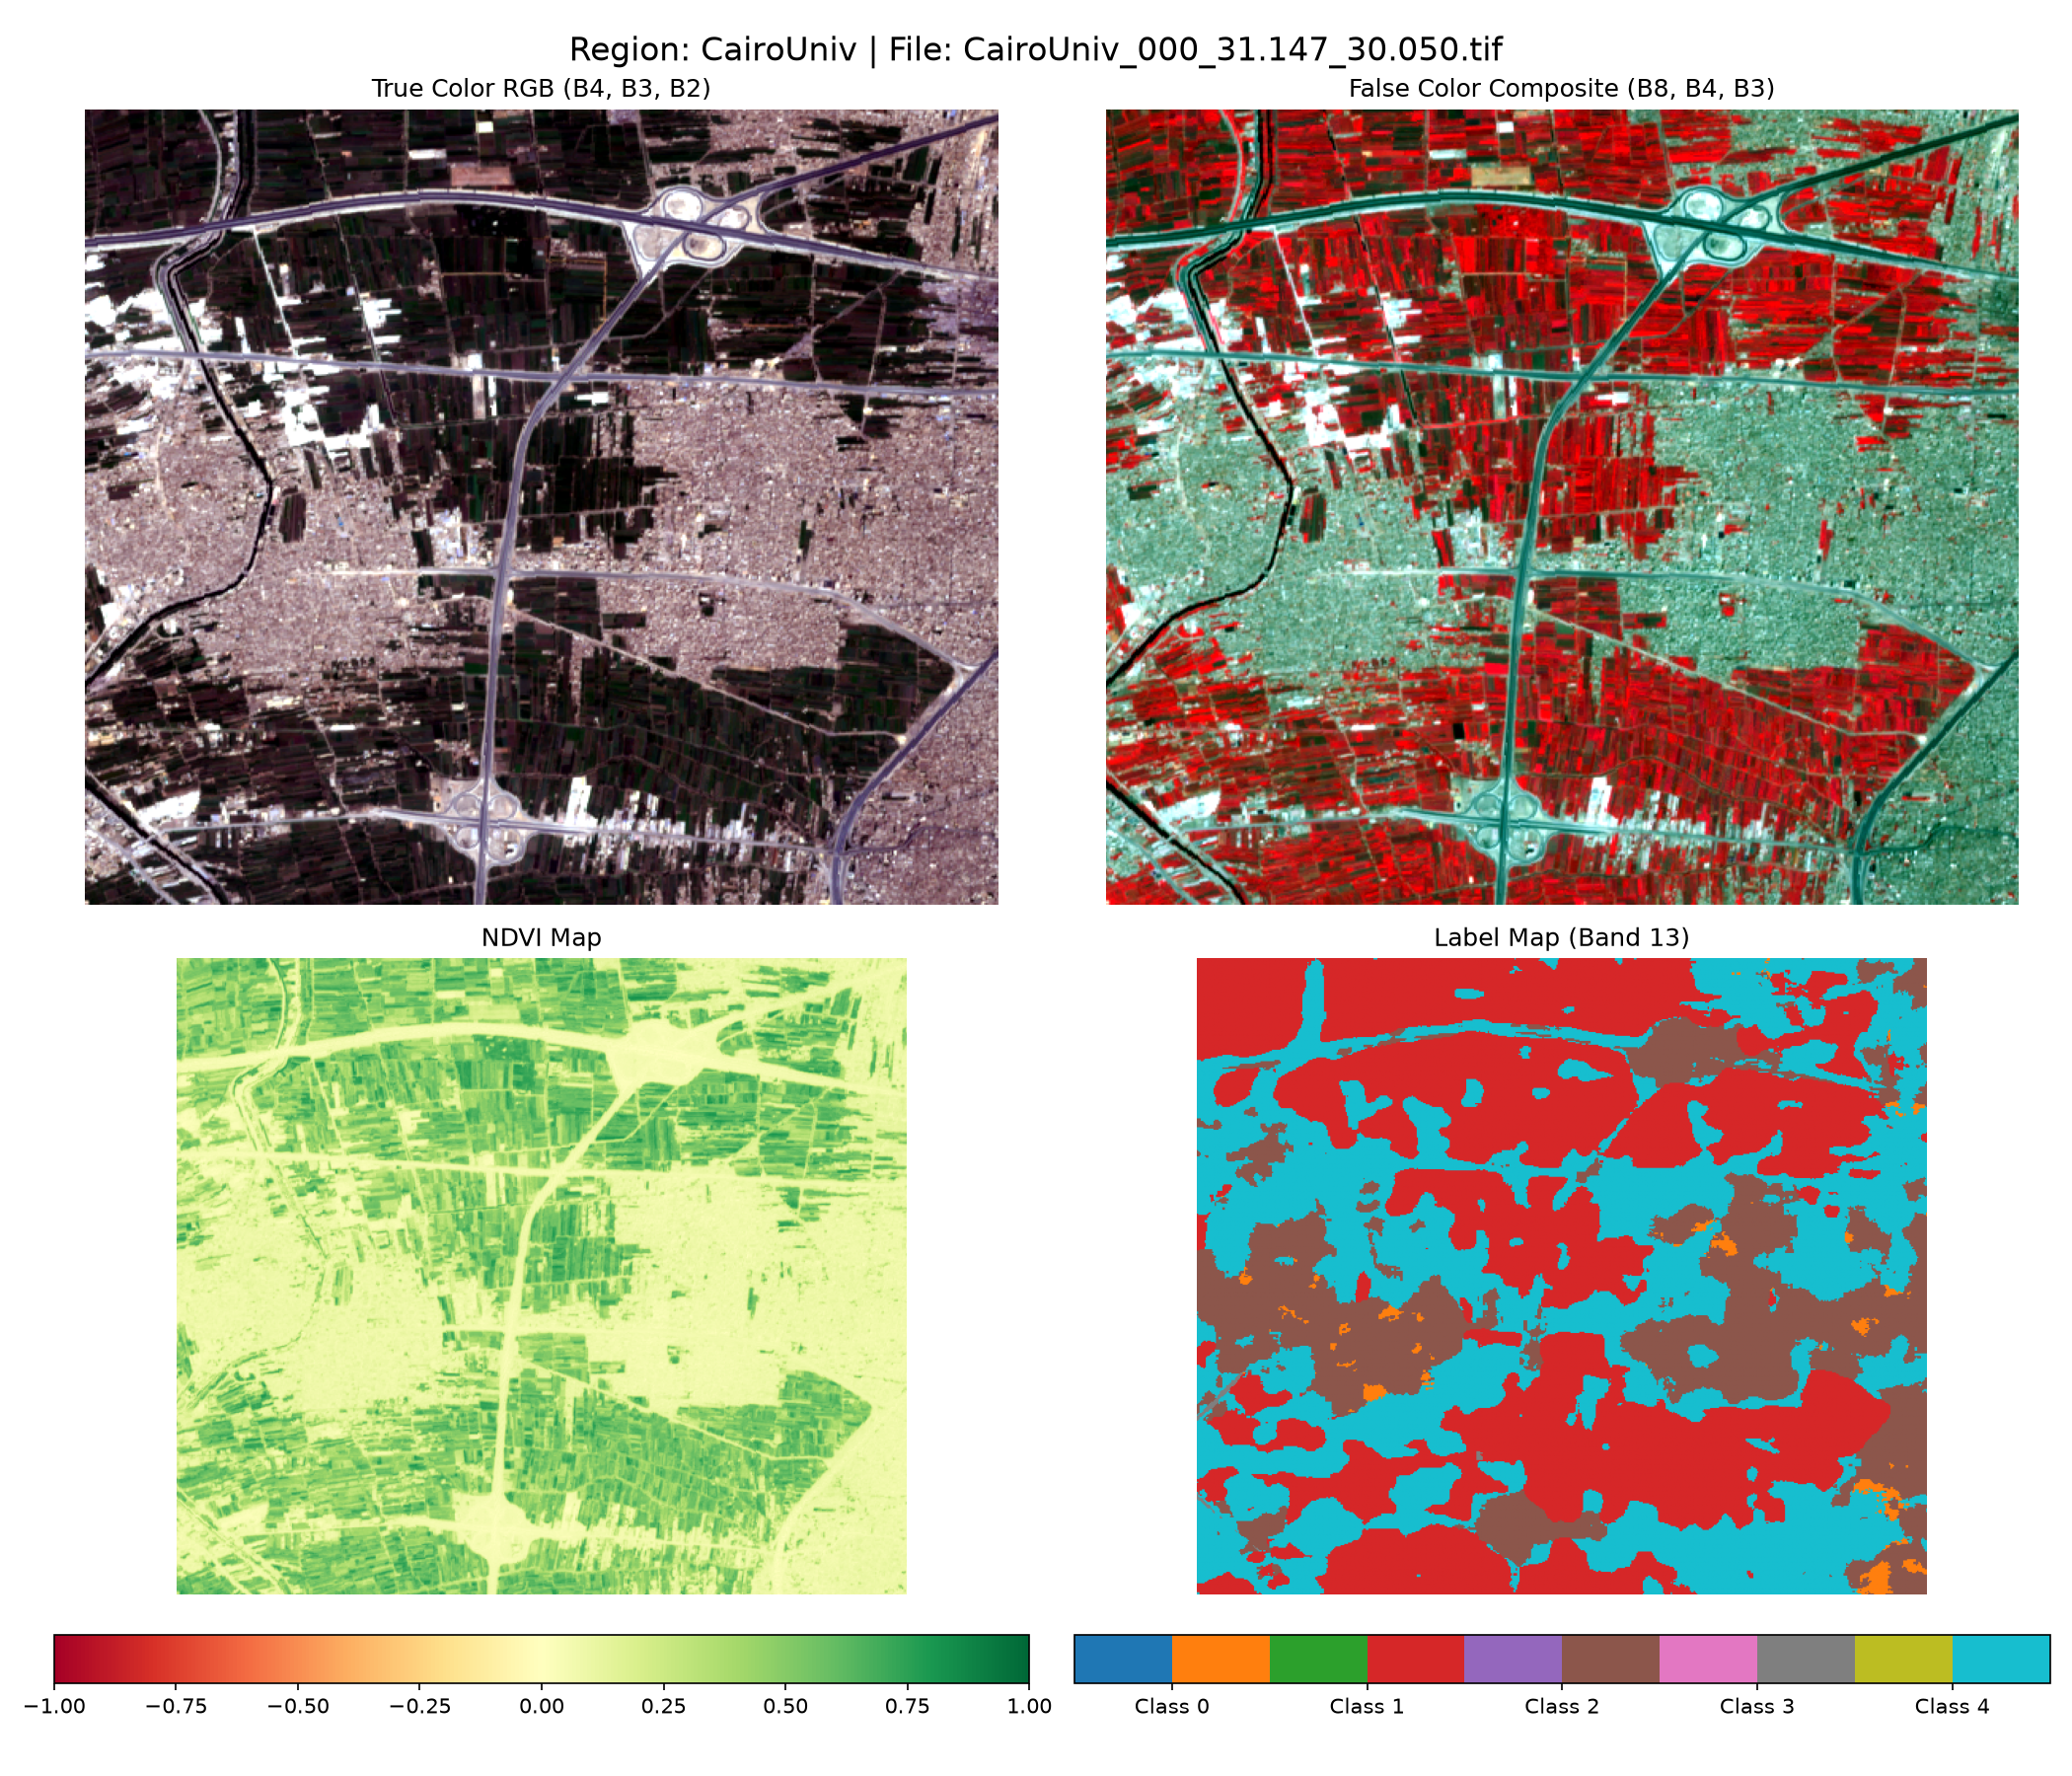
\includegraphics[width=0.9\textwidth]{figures/CairoUniv_visualization.png}
            \vskip0.1cm
            \footnotesize Cairo University Area Composite (RGB)
        \end{column}
    \end{columns}
\end{frame}

\section{Dataset \& Exploratory Data Analysis}
% Slide 4: Sentinel-2 Dataset & Class Mapping
\begin{frame}{Egypt Sentinel-2 Dataset \& Class Mapping}
    \begin{columns}
        \begin{column}{0.5\textwidth}
            \begin{block}{The Dataset Profile}
                \begin{itemize}
                    \item \textbf{Volume}: 719 multi-spectral GeoTIFF files (.tif).
                    \item \textbf{Dimensions}: $12 \text{ bands} \times 256 \times 256$ pixels.
                    \item \textbf{Labels}: Ground truth masks in Band 13.
                \end{itemize}
            \end{block}
            \begin{block}{Class Frequencies \& Semantics}
                \begin{itemize}
                    \item \textbf{0: Trees / Forest} (0.61\%) - rare canopy vegetation.
                    \item \textbf{1: Agriculture} (22.22\%) - Nile Valley / Delta.
                    \item \textbf{2: Desert / Soil} (51.80\%) - dominant class.
                    \item \textbf{3: Water Bodies} (8.37\%) - Nile river, lakes, sea.
                    \item \textbf{4: Urban / Roads} (17.00\%) - concrete/asphalt.
                \end{itemize}
            \end{block}
        \end{column}
        
        \begin{column}{0.5\textwidth}
            \centering
            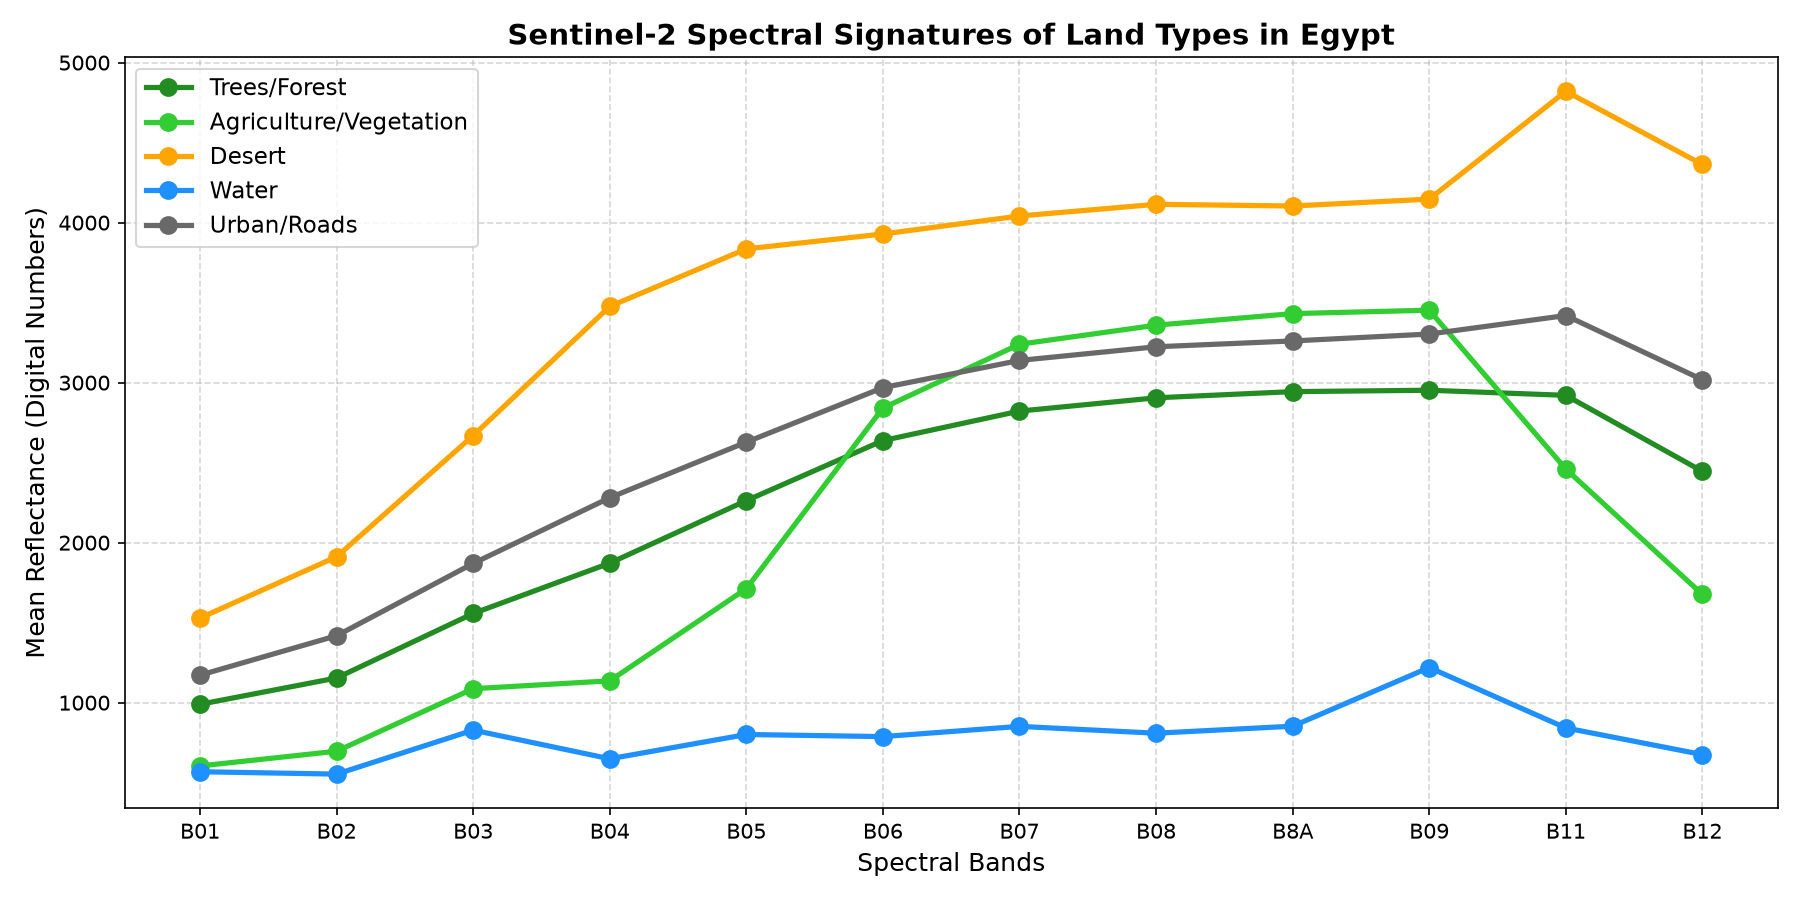
\includegraphics[width=0.95\textwidth]{figures/spectral_signatures.png}
            \vskip0.1cm
            \footnotesize Mean Spectral Signatures per Class
        \end{column}
    \end{columns}
\end{frame}

\section{Feature Engineering}
% Slide 5: Band Importance (Mutual Information)
\begin{frame}{Feature Engineering: Band Selection \& NDVI}
    \begin{columns}
        \begin{column}{0.5\textwidth}
            \begin{block}{Normalized Difference Vegetation Index (NDVI)}
                Calculated dynamically using NIR (B8) and Red (B4) bands:
                $$\text{NDVI} = \frac{\text{B08} - \text{B04}}{\text{B08} + \text{B04}}$$
                Highly discriminative for separating agriculture ($\text{NDVI} \approx 0.51$) from desert ($\text{NDVI} \approx 0.08$) and water ($\text{NDVI} \approx 0.01$).
            \end{block}
            \begin{block}{Mutual Information (MI) Insights}
                \begin{itemize}
                    \item Rank bands based on information gain.
                    \item \textbf{Top Features}: NIR (B8), SWIR-1 (B11), SWIR-2 (B12).
                    \item Validates that infrared bands are critical for semantic segmentation.
                \end{itemize}
            \end{block}
        \end{column}
        
        \begin{column}{0.5\textwidth}
            \centering
            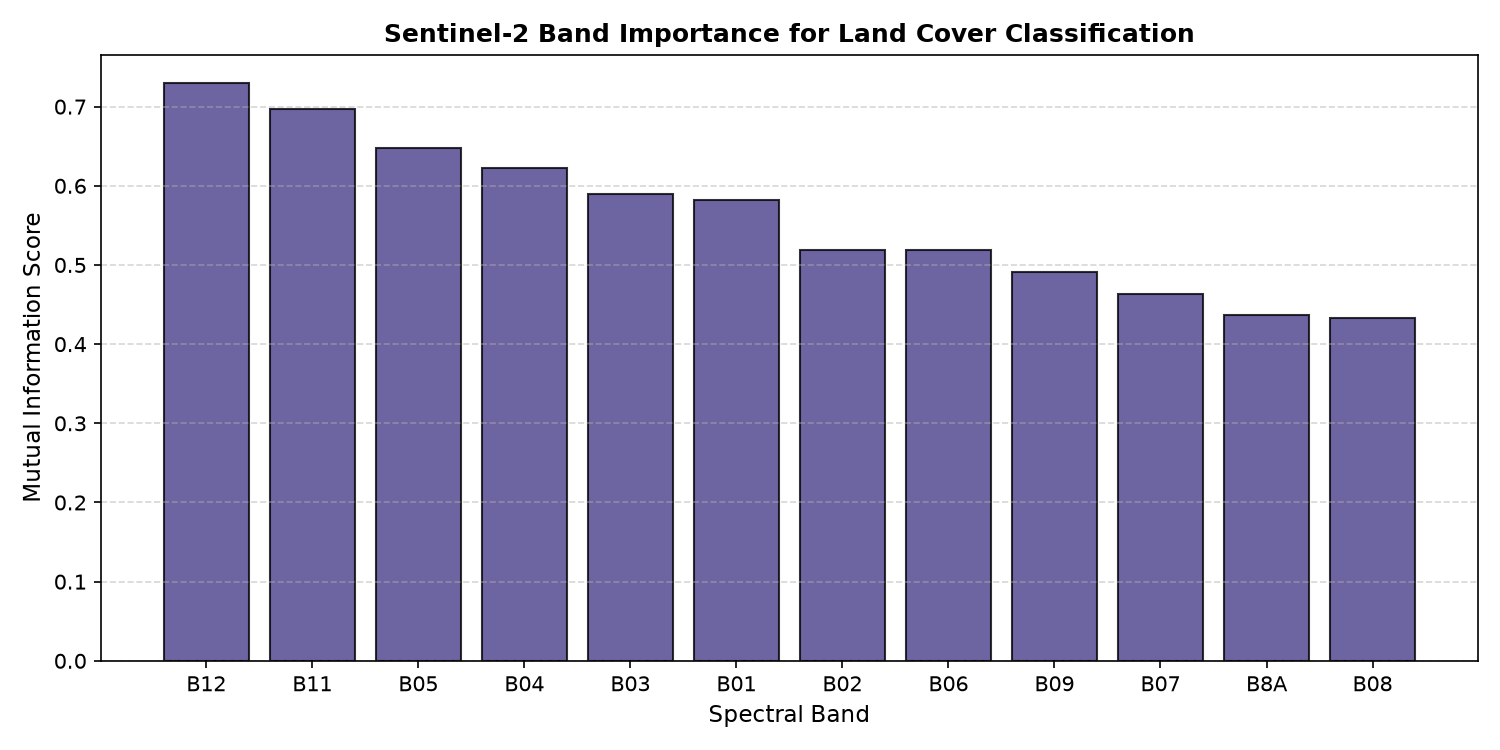
\includegraphics[width=0.95\textwidth]{figures/band_importance.png}
            \vskip0.1cm
            \footnotesize Mutual Information Scores per Band
        \end{column}
    \end{columns}
\end{frame}

% Slide 6: Principal Component Analysis (PCA)
\begin{frame}{Principal Component Analysis (PCA)}
    \begin{columns}
        \begin{column}{0.5\textwidth}
            \begin{block}{Dimensionality Reduction}
                \begin{itemize}
                    \item Standardized all 12 spectral bands.
                    \item Projected high-dimensional data onto orthogonal directions of maximum variance.
                    \item \textbf{Top 3 PCs} capture over 94\% of total variance.
                \end{itemize}
            \end{block}
            \begin{block}{Visualizing PCA (PC1 $\to$ R, PC2 $\to$ G, PC3 $\to$ B)}
                \begin{itemize}
                    \item Enhances environmental contrasts.
                    \item Separates dry sand, wet agricultural soil, salt basins, and urban infrastructure.
                \end{itemize}
            \end{block}
        \end{column}
        
        \begin{column}{0.5\textwidth}
            \centering
            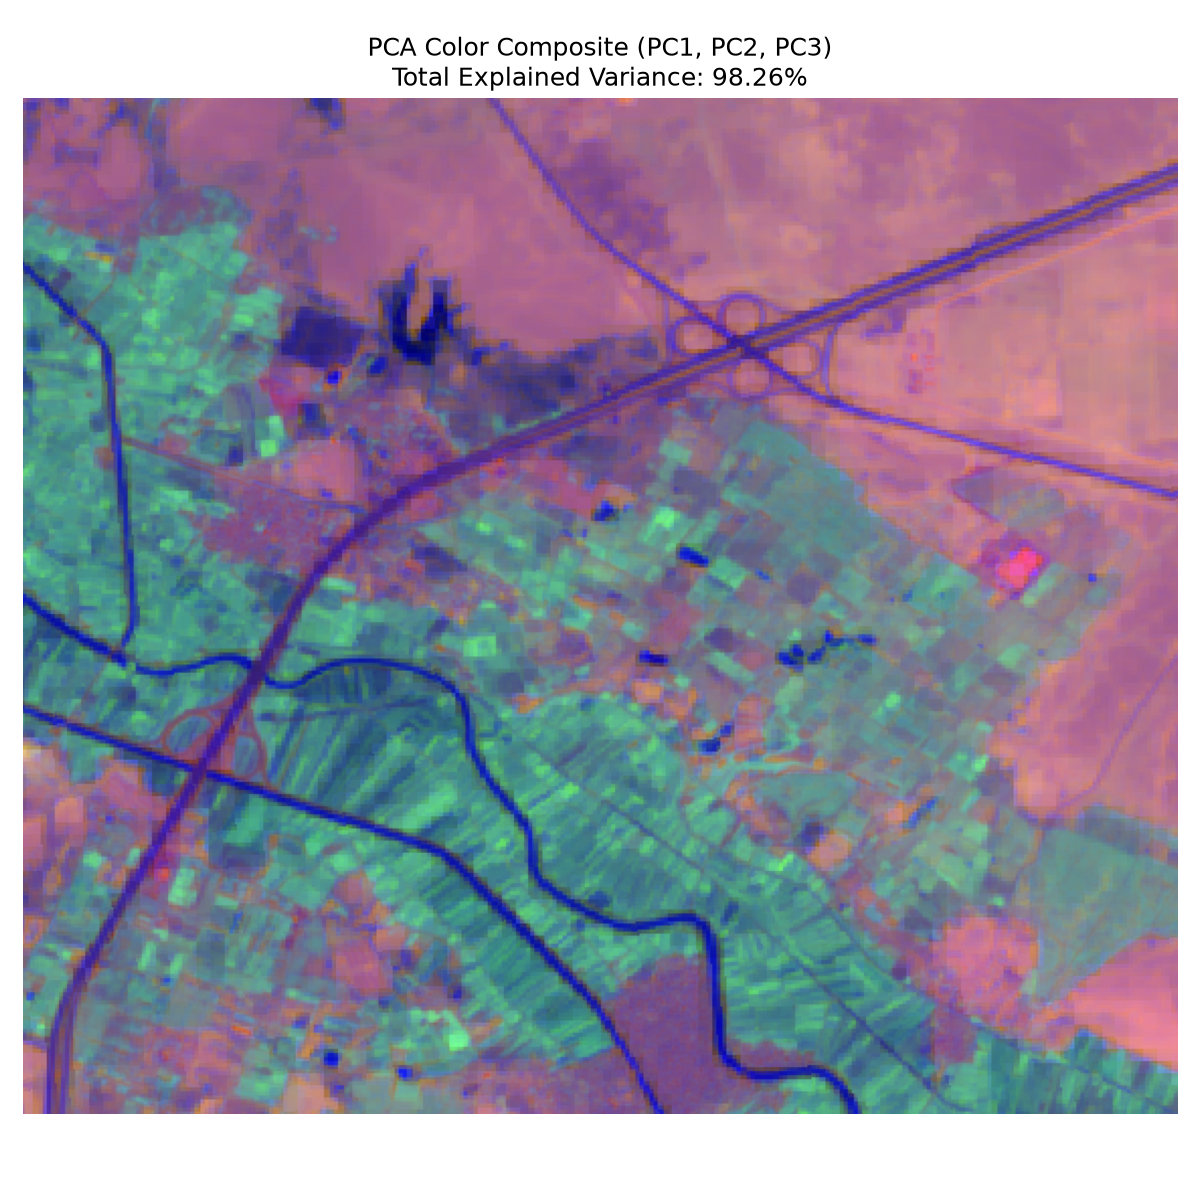
\includegraphics[width=0.8\textwidth]{figures/pca_composite.png}
            \vskip0.1cm
            \footnotesize False Color PCA Composite (PCs 1, 2, 3)
        \end{column}
    \end{columns}
\end{frame}

\section{Model Architecture}
% Slide 7: U-Net Architecture
\begin{frame}{U-Net Deep Learning Architecture}
    \begin{columns}
        \begin{column}{0.55\textwidth}
            \begin{block}{Model Architecture}
                \begin{itemize}
                    \item \textbf{Input}: 12 channels (multispectral bands) at $256 \times 256$ pixels.
                    \item \textbf{Contracting Encoder path}: Extract hierarchical spatial context via double convolutions, batch normalization, and max pooling.
                    \item \textbf{Expanding Decoder path}: Reconstruct resolution via up-convolutions.
                    \item \textbf{Skip Connections}: Concatenate high-resolution features from encoder to decoder to preserve sharp boundary details.
                    \item \textbf{Output}: 5-channel logit map (pixel-level class probabilities).
                \end{itemize}
            \end{block}
        \end{column}
        
        \begin{column}{0.42\textwidth}
            \centering
            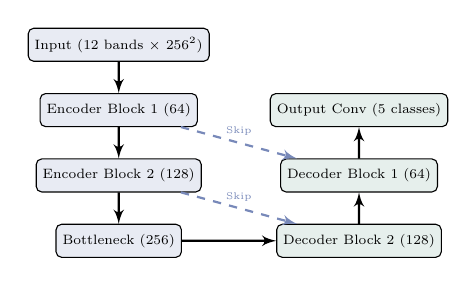
\begin{tikzpicture}[node distance=0.8cm, scale=0.7, every node/.style={scale=0.7}]
                \tikzstyle{box} = [draw, fill=navyblue!10, rectangle, minimum height=0.6cm, minimum width=2.2cm, text centered, rounded corners=2pt, font=\scriptsize]
                \tikzstyle{proc} = [draw, fill=emerald!10, rectangle, minimum height=0.6cm, minimum width=2.2cm, text centered, rounded corners=2pt, font=\scriptsize]
                \tikzstyle{line} = [draw, -latex', thick]
                
                \node [box] (in) {Input (12 bands $\times$ 256$^2$)};
                \node [box, below=0.4cm of in] (enc1) {Encoder Block 1 (64)};
                \node [box, below=0.4cm of enc1] (enc2) {Encoder Block 2 (128)};
                \node [box, below=0.4cm of enc2] (bridge) {Bottleneck (256)};
                \node [proc, right=1.2cm of bridge] (dec2) {Decoder Block 2 (128)};
                \node [proc, above=0.4cm of dec2] (dec1) {Decoder Block 1 (64)};
                \node [proc, above=0.4cm of dec1] (out) {Output Conv (5 classes)};
                
                \path [line] (in) -- (enc1);
                \path [line] (enc1) -- (enc2);
                \path [line] (enc2) -- (bridge);
                \path [line] (bridge) -- (dec2);
                \path [line] (dec2) -- (dec1);
                \path [line] (dec1) -- (out);
                
                % Skip connections
                \draw [line, dashed, navyblue!60] (enc2) -- node[above, font=\tiny]{Skip} (dec2);
                \draw [line, dashed, navyblue!60] (enc1) -- node[above, font=\tiny]{Skip} (dec1);
            \end{tikzpicture}
            \vskip0.1cm
            \footnotesize U-Net Information Flow
        \end{column}
    \end{columns}
\end{frame}

\section{Model Training \& Results}
% Slide 8: Training Configuration
\begin{frame}{Model Training \& Configuration}
    \begin{block}{Handling Severe Class Imbalance}
        Because desert covers 52\% of pixels and forest covers 0.6\%, we calculate \textbf{inverse-frequency weights} to scale the cross-entropy loss. Minority classes are penalized heavily:
        $$w_c = \frac{1}{\text{frequency}_c} \quad \text{scaled to sum to 1.0}$$
    \end{block}
    \begin{block}{Training Hyperparameters}
        \begin{itemize}
            \item \textbf{Optimiser}: AdamW (weight decay = $1\text{e-}4$) for robust regularization.
            \item \textbf{Scheduler}: Cosine Annealing Learning Rate (starts at $1\text{e-}3$, decays to $1\text{e-}6$).
            \item \textbf{Epochs}: 10 (fully trained on CUDA GPU).
            \item \textbf{Splits}: Region-stratified: 70\% Train (503 images), 15\% Val (108), 15\% Test (108).
        \end{itemize}
    \end{block}
\end{frame}

% Slide 9: Metrics & Loss Curves
\begin{frame}{Training Curves \& Performance Metrics}
    \begin{columns}
        \begin{column}{0.5\textwidth}
            \begin{block}{Performance Metrics Achieved}
                \begin{itemize}
                    \item \textbf{Overall Pixel Accuracy}: \textbf{89.36\%}
                    \item \textbf{Mean Intersection over Union (mIoU)}: \textbf{69.46\%}
                \end{itemize}
            \end{block}
            \begin{block}{Class-specific IoU Scores}
                \begin{itemize}
                    \item \textbf{Water Bodies}: \textbf{92.68\%} (Excellent)
                    \item \textbf{Desert / Bare Soil}: \textbf{87.03\%} (Strong)
                    \item \textbf{Agriculture / Vegetation}: \textbf{86.75\%} (Strong)
                    \item \textbf{Urban / Roads}: \textbf{65.11\%} (Moderate)
                    \item \textbf{Trees / Forest}: \textbf{15.74\%} (Challenging due to scarcity)
                \end{itemize}
            \end{block}
        \end{column}
        
        \begin{column}{0.5\textwidth}
            \centering
            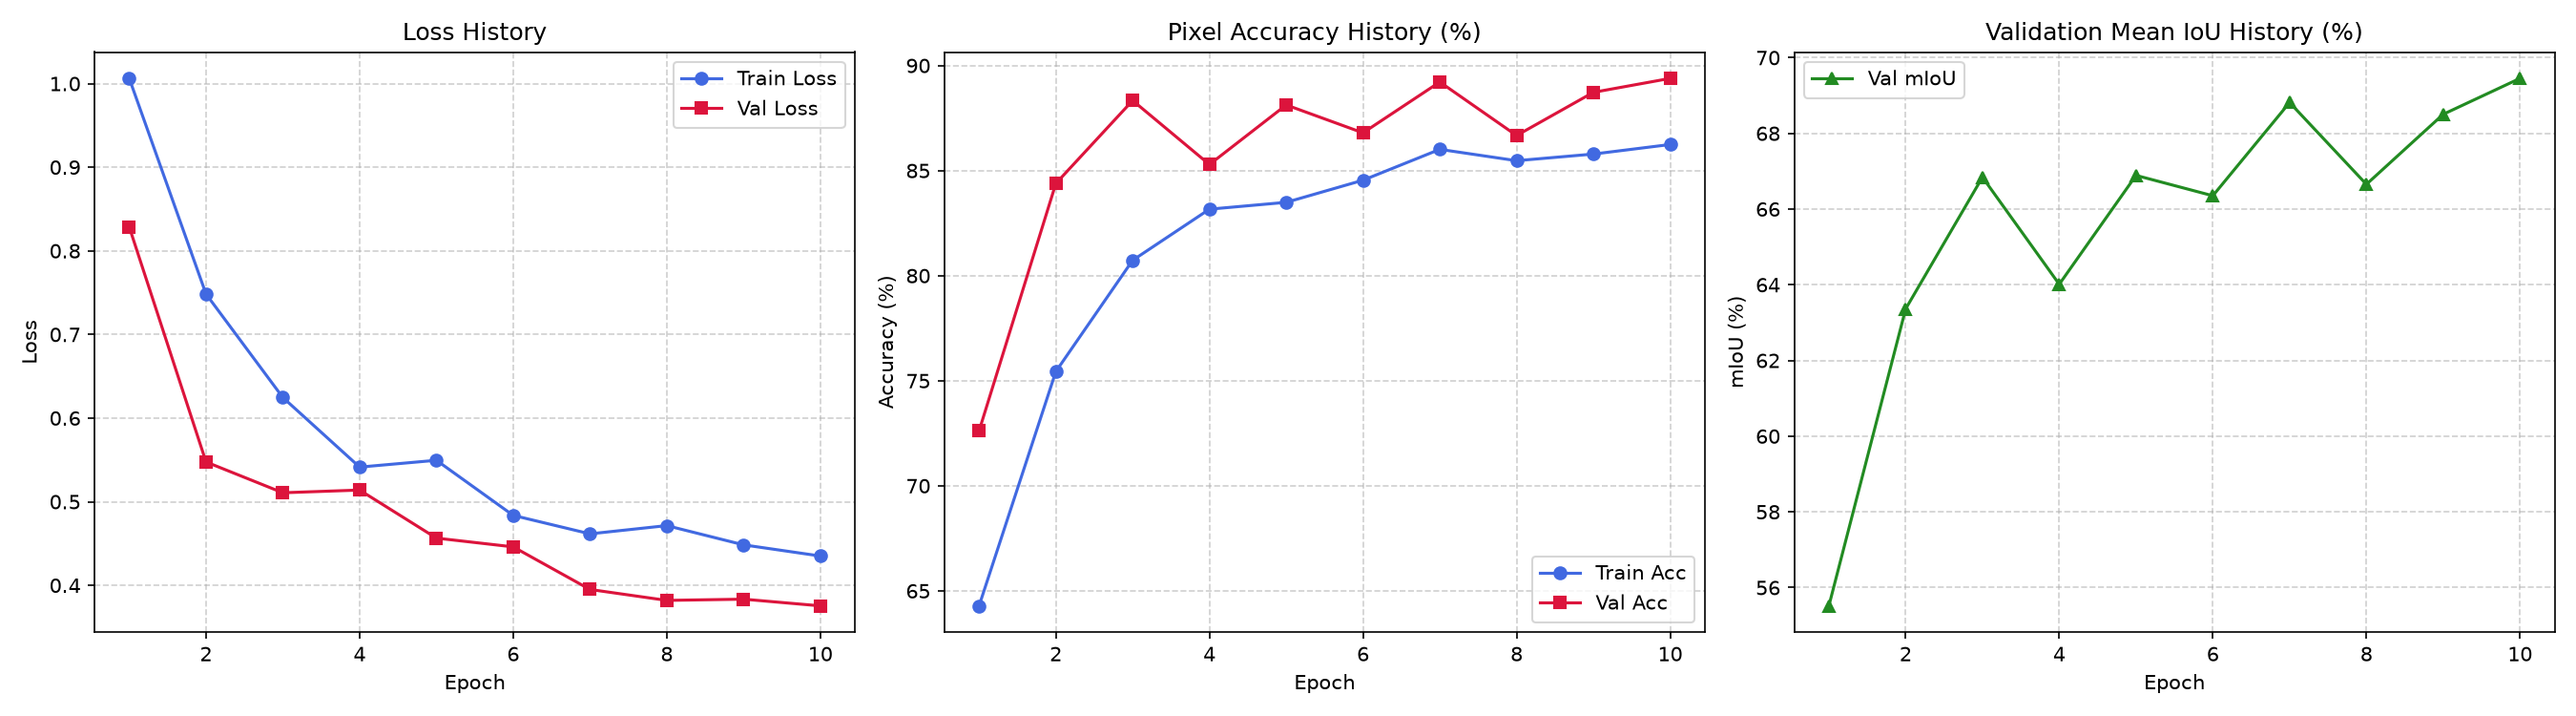
\includegraphics[width=0.95\textwidth]{figures/training_learning_curves.png}
            \vskip0.1cm
            \footnotesize Loss \& mIoU convergence over 10 Epochs
        \end{column}
    \end{columns}
\end{frame}

% Slide 10: Visual Predictions
\begin{frame}{Qualitative Results: Semantic Segmentation Maps}
    \centering
    \begin{columns}
        \begin{column}{0.33\textwidth}
            \centering
            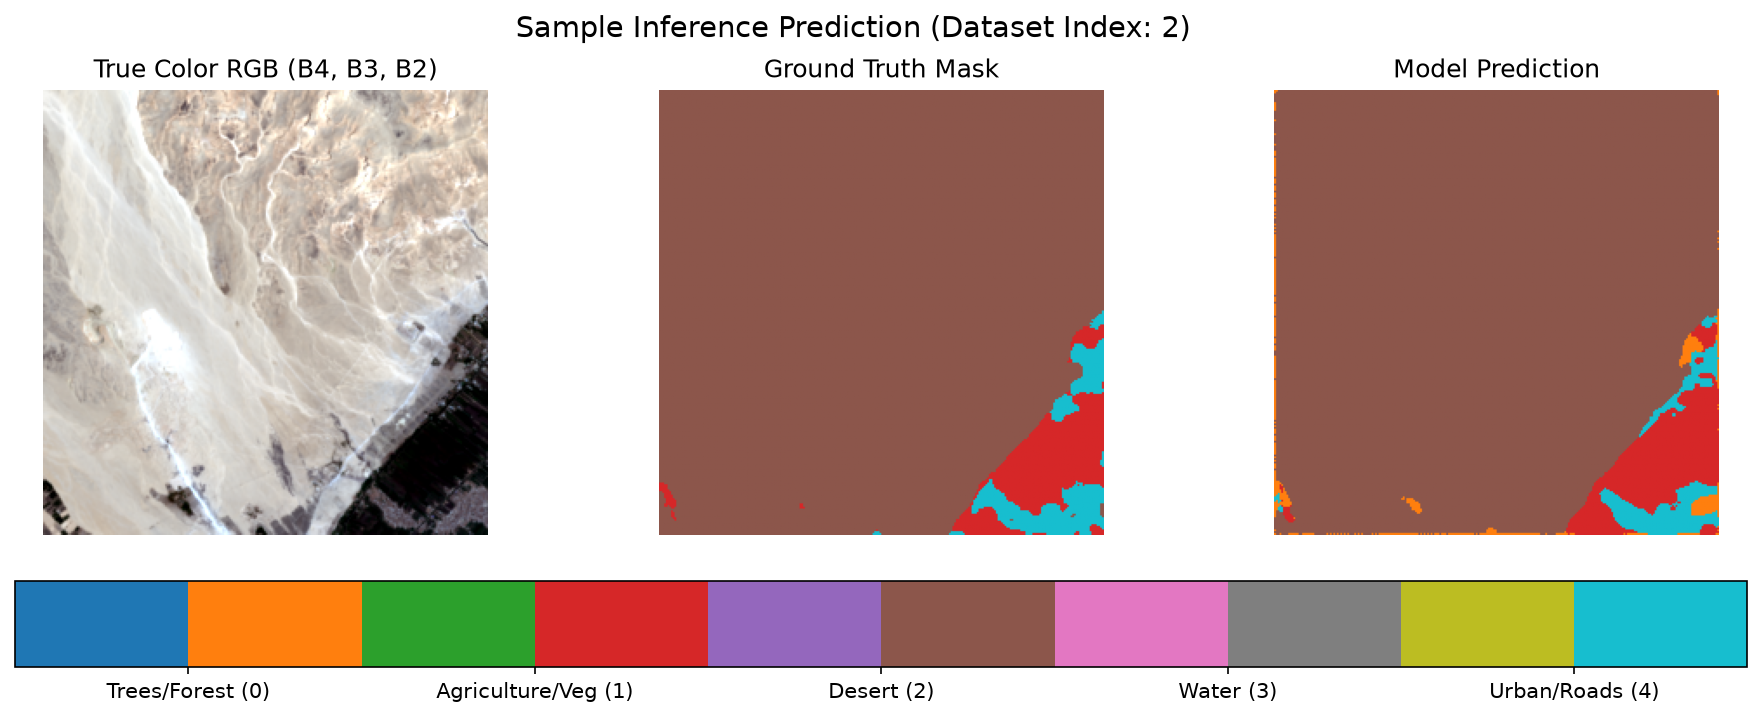
\includegraphics[width=0.9\textwidth]{figures/prediction_sample_1.png}
            \vskip0.1cm
            \footnotesize Nile Delta Agricultural Grid
        \end{column}
        \begin{column}{0.33\textwidth}
            \centering
            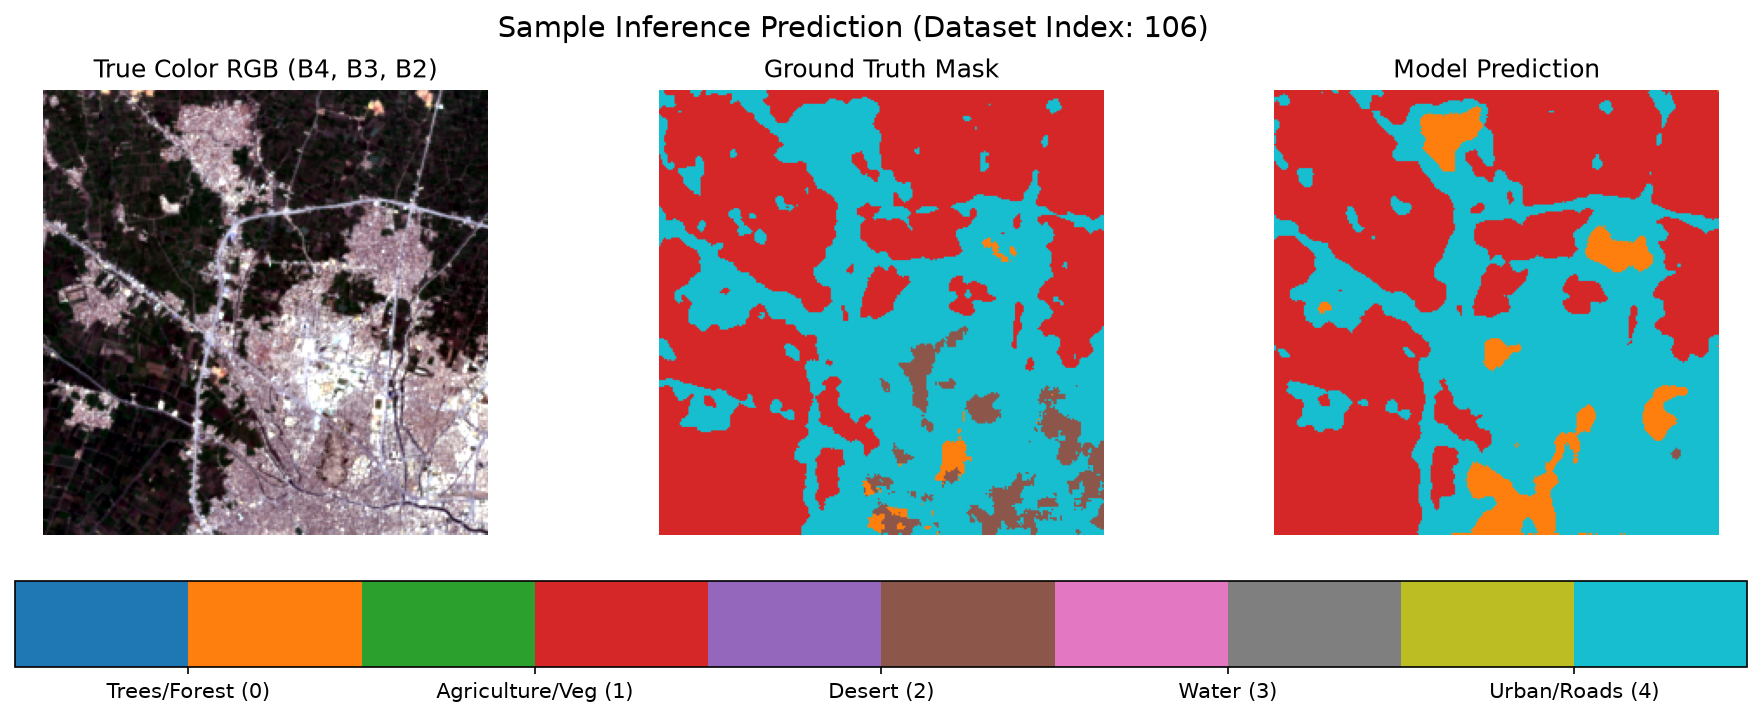
\includegraphics[width=0.9\textwidth]{figures/prediction_sample_2.png}
            \vskip0.1cm
            \footnotesize Suez Canal (Water vs Desert)
        \end{column}
        \begin{column}{0.33\textwidth}
            \centering
            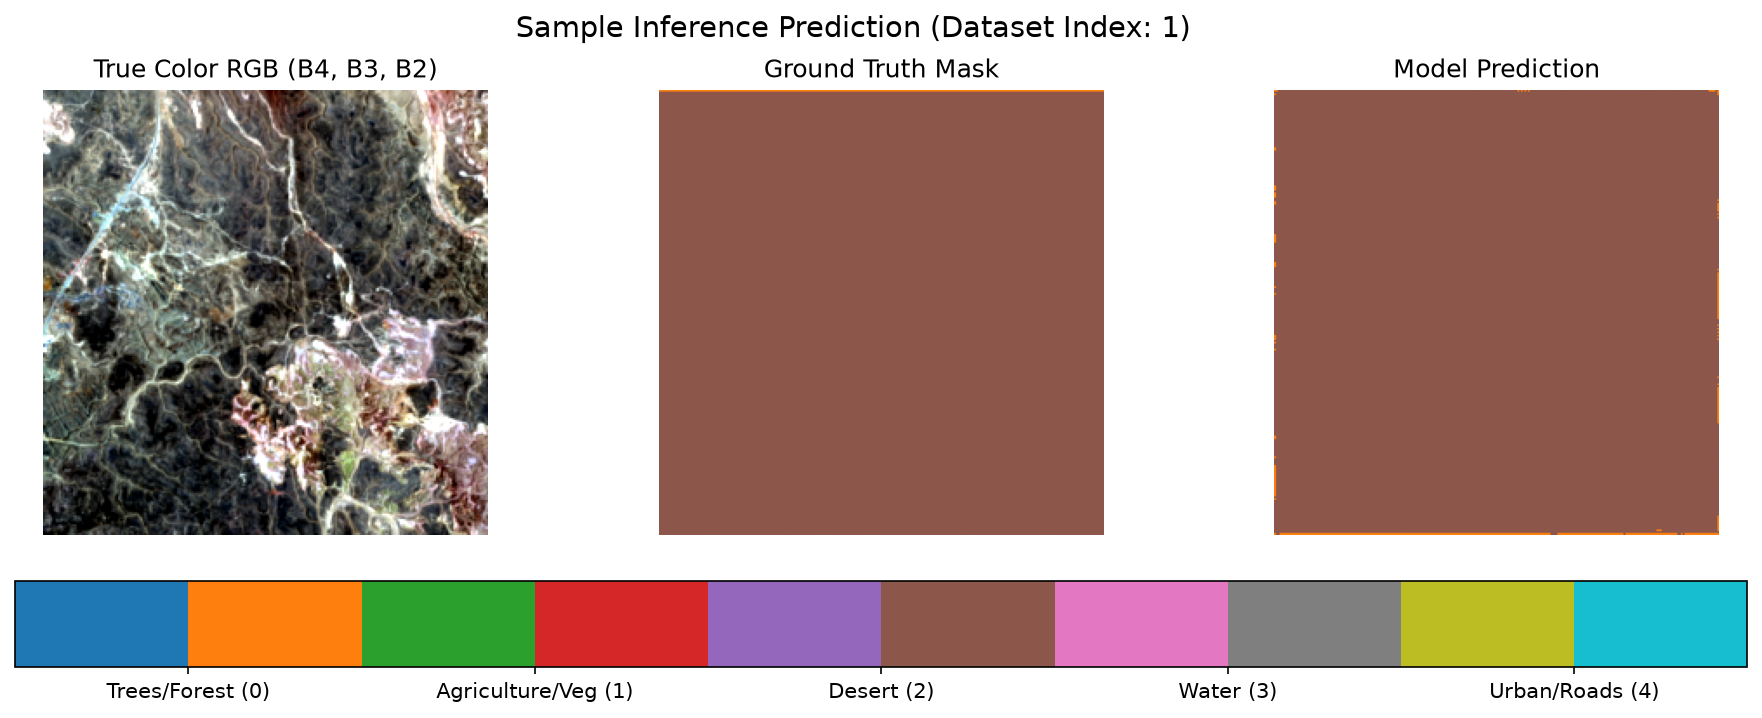
\includegraphics[width=0.9\textwidth]{figures/prediction_sample_3.png}
            \vskip0.1cm
            \footnotesize Cairo Urban Expansion
        \end{column}
    \end{columns}
\end{frame}

\section{Deployment: Interactive Dashboard}
% Slide 11: Web App GUI & Architecture
\begin{frame}{Deployment: SentinelVision Web Application}
    \begin{columns}
        \begin{column}{0.55\textwidth}
            \begin{block}{System Architecture}
                \begin{itemize}
                    \item \textbf{Backend}: FastAPI (Python) server.
                    \item \textbf{Frontend}: Single-page HTML5 dashboard styled with Tailwind CSS, leveraging Plotly.js for interactive charts.
                    \item \textbf{Inference}: GeoTIFF upload $\to$ memory stream $\to$ U-Net evaluation $\to$ Plotly charts generated on the fly.
                \end{itemize}
            \end{block}
            \begin{block}{Plotly Charts Generated}
                \begin{itemize}
                    \item \textbf{True Color composite}: stretched Red/Green/Blue bands.
                    \item \textbf{Classification Map}: Heatmap aligned with class colors.
                    \item \textbf{Bar Chart}: Percentage area breakdown.
                \end{itemize}
            \end{block}
        \end{column}
        
        \begin{column}{0.4\textwidth}
            \centering
            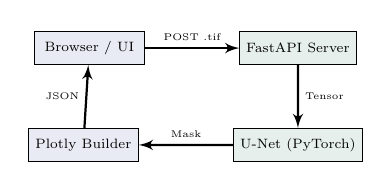
\begin{tikzpicture}[node distance=1cm, scale=0.7, every node/.style={scale=0.7}]
                \tikzstyle{c} = [draw, fill=navyblue!10, rectangle, minimum height=0.6cm, minimum width=2cm, font=\scriptsize]
                \tikzstyle{s} = [draw, fill=emerald!10, rectangle, minimum height=0.6cm, minimum width=2cm, font=\scriptsize]
                \tikzstyle{l} = [draw, -latex', thick]
                
                \node [c] (ui) {Browser / UI};
                \node [s, right=1.2cm of ui] (api) {FastAPI Server};
                \node [s, below=0.8cm of api] (model) {U-Net (PyTorch)};
                \node [c, left=1.2cm of model] (plotly) {Plotly Builder};
                
                \draw [l] (ui) -- node[above, font=\tiny]{POST .tif} (api);
                \draw [l] (api) -- node[right, font=\tiny]{Tensor} (model);
                \draw [l] (model) -- node[above, font=\tiny]{Mask} (plotly);
                \draw [l] (plotly) -- node[left, font=\tiny]{JSON} (ui);
            \end{tikzpicture}
            \vskip0.2cm
            \footnotesize GUI System Information Flow
        \end{column}
    \end{columns}
\end{frame}

\section{Summary \& Conclusion}
% Slide 12: Conclusion
\begin{frame}{Conclusion \& Future Scope}
    \begin{block}{Summary of Achievements}
        \begin{itemize}
            \item Successfully built and trained a multispectral (12-band) U-Net segmentation model achieving \textbf{89.36\% accuracy} and \textbf{69.46\% mIoU}.
            \item Addressed class imbalance using normalized inverse-frequency weighted cross-entropy.
            \item Deployed the model on an interactive web dashboard with zero disk-write footprint.
        \end{itemize}
    \end{block}
    \begin{block}{Future Enhancements}
        \begin{itemize}
            \item Use transformer-based architectures (e.g. SegFormer) for improved road/urban boundary accuracy.
            \item Expand the dataset to include multitemporal seasonal imagery of Egypt.
            \item Deploy on cloud instances like Google Cloud Run or AWS EC2 for public access.
        \end{itemize}
    \end{block}
\end{frame}

% Slide 13: Thank you
\begin{frame}
    \centering
    \Huge \color{navyblue} Thank You!
    \vskip1cm
    \Large Questions \& Discussion
\end{frame}

\end{document}
